\chapter{WebAssembly Serverless Platform Design}
\label{chap:poc}

In this chapter, the proof of concept for a simple \gls{serverless} compute platform using WebAssembly technology will be explored. For simplicity, the platform runs on an HTTP server to redirect HTTP requests to specific WebAssembly modules. For this, we will use Wasmtime \cite{bytecodealliance_2022_wasmtime} as the WebAssembly runtime, but we could also use Wasmer \cite{wasmerinc_2023_wasmer}. Since Wasmtime does only have Rust integration, we will use the Rust language along with the popular Rust web framework, "Actix-web \cite{actixteam_actix}", due to its lightweight and fast nature. As mentioned in the previous chapter, Wasmtime offers excellent support for the latest WASI standards and features. 

As Figure \ref{fig:poc} illustrates, this proof of concept assumes that there will be a function registry service that stores the ahead-of-time compiled \gls{WebAssembly} binaries. Additionally, a serverless platform needs to be distributed; therefore, API gateways and load balancers are necessary to serve requests across the network. Nonetheless, this proof of concept primarily focuses on the WebAssembly aspect of the platform, leaving the deployment platform, API gateway and load balancers outside the scope of the discussion. 
%
\begin{figure}[htbp]
	\centering
		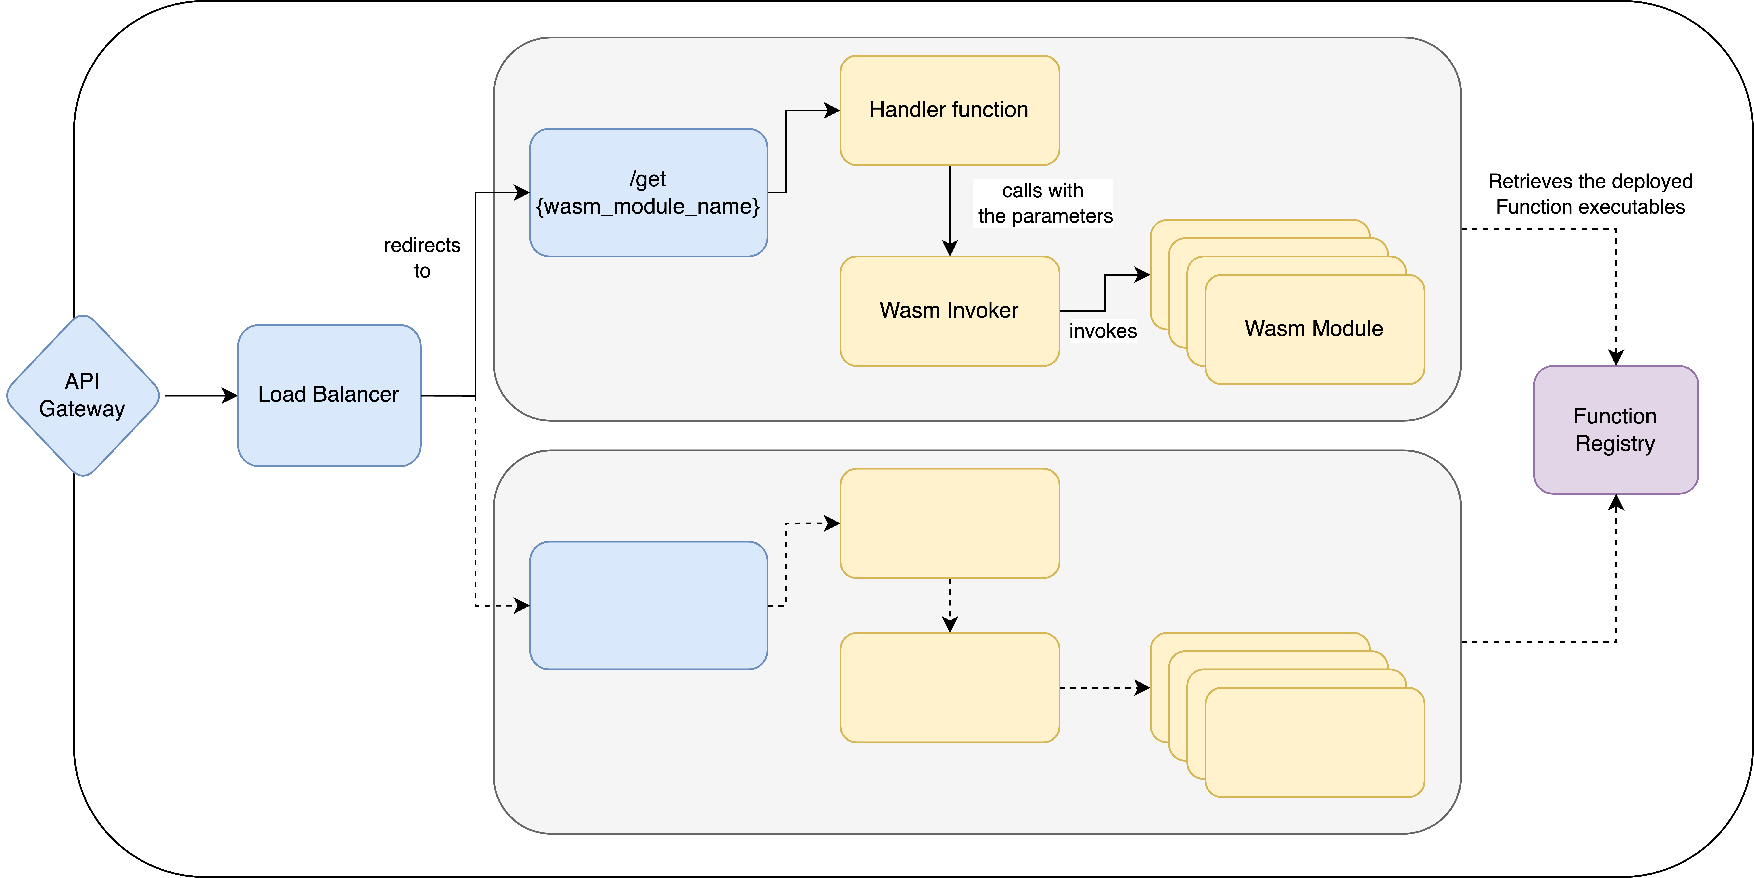
\includegraphics[width=1\linewidth]{images/poc/poc.pdf}
	\caption{Execution flow of the simple POC serverless platform, inspired by \cite[p. 142]{gackstatter_2022_pushing}}
	\label{fig:poc}
\end{figure}
%
The platform has a single endpoint that accepts HTTP requests with a Wasm module name in the path and query parameters. The endpoint will then load the Wasm module from the same directory and call the defined \texttt{invoke\_wasm\_module} in listing \ref{lst:poc-invocation}. This function is the main part of our platform, it is responsible for creating a Wasmtime runtime engine and linker, adding the WASI APIs to the linker. The function then creates a WASI context with the query parameters and loads the module with the file name. The linker is used to link the Wasm module with the later created instance together. There is also a buffer that will be used to store the response from the Wasm module.
%
\begin{lstlisting}[frame=lines, style=Rust, caption={invocation function}, showstringspaces=false, label={lst:poc-invocation}, captionpos=b]
fn invoke_wasm_module(wasm_module_name: String, params: HashMap<String, String>) -> Result<String> {
    let engine = Engine::default();
    let mut linker = Linker::new(&engine);
    wasmtime_wasi::add_to_linker(&mut linker, |s| s)?;

    let stdout_vec_buf: Vec<u8> = vec![]; // a buffer that will contain the response
    let stdout_vec_mutex = Arc::new(RwLock::new(stdout_vec_buf));
    let stdout = WritePipe::from_shared(stdout_vec_mutex.clone());

    // params to array
    let envs: Vec<(String, String)> = params
        .iter()
        .map(|(key, value)| (key.clone(), value.clone()))
        .collect();

    let wasi = WasiCtxBuilder::new()
        .stdout(Box::new(stdout))
        .envs(&envs)?
        .build();
    let mut store = Store::new(&engine, wasi);

    let module = Module::from_file(&engine, &wasm_module_name)?;
    linker.module(&mut store, &wasm_module_name, &module)?;

    run_wasm_module(&mut store, &module, &linker).unwrap();

    // get the response
    let mut buffer: Vec<u8> = Vec::new();
    stdout_vec_mutex
        .read()
        .unwrap()
        .iter()
        .for_each(|i| buffer.push(*i));

    let s = String::from_utf8(buffer)?;
    Ok(s)
}
\end{lstlisting}
%
Directly after, we then call the \texttt{run\_wasm\_module} function shown in listing \ref{lst:poc-start}. This is where the linker links the module with the newly created instance. The instance is used to search for the start function, the "\_start" function is the starting point of the Wasm modules. It will call the function and return the result. The result is then stored in the buffer and returned to the caller.
%
\begin{lstlisting}[frame=lines, style=Rust, caption={calling the wasm start function}, showstringspaces=false, label={lst:poc-start}, captionpos=b]
fn run_wasm_module(
    mut store: &mut Store<WasiCtx>,
    module: &Module,
    linker: &Linker<WasiCtx>,
) -> Result<()> {
    let instance = linker.instantiate(&mut store, module)?;
    let instance_main = instance.get_typed_func::<(), ()>(&mut store, "_start")?;
    Ok(instance_main.call(&mut store, ())?)
}
\end{lstlisting}
%
To test the platform, we can use any WASI complaint Wasm binary. The following AssemblyScript file contains a simple statement that outputs "Hello World!" on the terminal. The AssemblyScript compiler will compile the file to a WASI complaint Wasm binary. For this we will also need the "wasi-shim" which is a standalone dependency.
%
\begin{lstlisting}[frame=lines, style=JavaScript, caption={AssemblyScript file with a simple console output}, showstringspaces=false, label={lst:as-hello-world}, captionpos=b]
// calling AssemblyScript's console.log, 
// which calls the corresponding WASI interface
console.log('Hello World!');
\end{lstlisting}

\section{Wind-up}

This example shows how easy it is to create a simple \gls{serverless} platform that can invoke any WASI complaint Wasm module. The above Wasm module example was written in AssemblyScript, but in fact, we can use any language that compiles to Wasm and its WASI complaint. If we build this project with the highest compiler optimization, then the resulting binary is only 15 MB in size. This is a modest size for a serverless platform, with less than 80 lines of code. If we run the server and call the mentioned "hello-world" example, we get the following result:
\begin{lstlisting}[frame=lines]
curl -w %{time_total}\\n  http://localhost:8000/hello-world
Hello World!
0.009886
\end{lstlisting}

The result contains the response which, in this case is "Hello World!" and the measured time until the response was received. The measured time is around 10 milliseconds and a deviation of ±15\%. The response time is quite fast, but we should consider the following points:
\begin{itemize}
    \item The server is running on a local machine, therefore it does not take dns lookup, tcp handshake, load balancing overhead and other network related overheads into account
    \item The system has more resources (M1 Pro CPU and 32 GB RAM) than a typical \gls{edge computing} device
    \item The server lacks various features typically associated with a \gls{serverless} platform, therefore it has less overhead than a typical serverless platform
    \item The Wasm module is very simple and does not contain any heavy computation
    \item The large portion of the response time is caused by the Actix Web framework
\end{itemize}

To concrete the last point, we can run the same test without the Wasmtime runtime and the Wasm module. This time we will use the Actix Web framework to return the "Hello World!" string directly and we use the same optimization level as before. The result is shown in the following listing:

\begin{lstlisting}[frame=lines]
curl -w %{time_total}\\n  http://localhost:8000/hello-world
Hello world!
0.005646
\end{lstlisting}

This time the response time is around 6 milliseconds with a deviation of ±10\%. This shows that the Actix Web framework is responsible for 60\% of the response time compared to the previous test setup. This is not surprising, as the Actix Web framework is a full-fledged web framework with many features. 

This is as an excellent starting point for running more precise measurements on the actual runtime in the next chapter, with the aim of gathering a more better picture of the performance of various factors.
